\documentclass[12pt,a4paper]{article}
\usepackage{amsmath,amscd,amsbsy,amssymb,latexsym,url,bm,amsthm}
\usepackage{epsfig,graphicx,subfigure}
\usepackage{enumitem,balance}
\usepackage{wrapfig}
\usepackage{mathrsfs,euscript}
\usepackage[usenames]{xcolor}
\usepackage{hyperref}
\usepackage[vlined,ruled,linesnumbered]{algorithm2e}
\hypersetup{colorlinks=true,linkcolor=black}

\newtheorem{theorem}{Theorem}
\newtheorem{lemma}[theorem]{Lemma}
\newtheorem{proposition}[theorem]{Proposition}
\newtheorem{corollary}[theorem]{Corollary}
\newtheorem{exercise}{Exercise}
\newtheorem*{solution}{Solution}
\newtheorem{definition}{Definition}
\theoremstyle{definition}

\renewcommand{\thefootnote}{\fnsymbol{footnote}}

\newcommand{\postscript}[2]
 {\setlength{\epsfxsize}{#2\hsize}
  \centerline{\epsfbox{#1}}}

\renewcommand{\baselinestretch}{1.0}

\setlength{\oddsidemargin}{-0.365in}
\setlength{\evensidemargin}{-0.365in}
\setlength{\topmargin}{-0.3in}
\setlength{\headheight}{0in}
\setlength{\headsep}{0in}
\setlength{\textheight}{10.1in}
\setlength{\textwidth}{7in}
\makeatletter \renewenvironment{proof}[1][Proof] {\par\pushQED{\qed}\normalfont\topsep6\p@\@plus6\p@\relax\trivlist\item[\hskip\labelsep\bfseries#1\@addpunct{.}]\ignorespaces}{\popQED\endtrivlist\@endpefalse} \makeatother
\makeatletter
\renewenvironment{solution}[1][Solution] {\par\pushQED{\qed}\normalfont\topsep6\p@\@plus6\p@\relax\trivlist\item[\hskip\labelsep\bfseries#1\@addpunct{.}]\ignorespaces}{\popQED\endtrivlist\@endpefalse} \makeatother

\begin{document}
\noindent

%========================================================================
\noindent\framebox[\linewidth]{\shortstack[c]{
\Large{\textbf{Lab02-Divide and Conquer}}\vspace{1mm}\\
CS214-Algorithm and Complexity, Xiaofeng Gao, Spring 2020.}}
\begin{center}
\footnotesize{\color{red}$*$ If there is any problem, please contact TA Yiming Liu.}

% Please write down your name, student id and email.
\footnotesize{\color{blue}$*$ Name: Yulong Hui \quad Student ID: 518030910059 \quad Email: qinchuanhuiyulong@sjtu.edu.cn}
\end{center}

\begin{enumerate}
    \item
    \textbf{Quicksort} is based on the Divide-and-Conquer method. Here is the two-step divide-and-conquer process for sorting a typical subarray $A[p \ldots r]$:
    \begin{enumerate}

    	\item
    	\textbf{Divide:} Partition the array $A[p \ldots r]$ into two subarrays $A[p \ldots q-1]$ and $A[q+1 \ldots r]$ such that each element of $A[p \ldots q-1]$ is less than or equal to $A[q],$ which is, in turn, less than or equal to each element of $A[q+1 \ldots r].$ Compute the index $q$ as part of this partitioning procedure.
    	
    	\item
    	\textbf{Conquer:} Sort $A[p \ldots q-1]$ and $A[q+1 \ldots r]$ respectively by recursive calls to Quicksort.
    	
    \end{enumerate}
    Write down the recurrence function $T(n)$ of QuickSort and compute its time complexity.

    {\color{purple}Hint: At this time $T(n)$ is split into two subarrays with different sizes (usually), and you need to describe its recurrence relation by the sum of two subfunctions plus additional operations.}
    
    \begin{solution}
     Every time we want to divide the array of $n$ elements, there should be comparisons of $\Theta(n)$.
     
     \textbf{Best.} When it comes to the best case, the two subarrays should have the same number of elements of $n/2$. Then, we can get:
       $$T(n)=2T(n/2)+\Theta(n)$$
       Because ${2}/{2^1}=1$, the $T(n)$ should be $\Theta(n\log n)$.
       
        Due to the best case, it can be expressed as $\Omega((r-p+1) \times log (r-p+1) )$
       
     \textbf{Average.} We use the equation below:  $$T(n)=n-1+T(i-1)+T(n-i)\qquad (n\geq2)$$
     Obviously, $$T(1)=0 \quad T(2)=1 \eqno(1)$$.
     
     Considering the average condition, we should think the possiblity of the value of $i$. Assume that the value of i between 1 and n is equally possible. So we can get an average $T(n)$ :
     $$T(n)=n-1+\frac{1}{n}\times\displaystyle \sum^{n}_{i=1}{[T(i-1)+T(n-i)]}.\eqno(2)$$
     $$T(n)=n-1+\frac{2}{n}\times\displaystyle \sum^{n-1}_{i=1}{T(i)}.\eqno(3)$$
     Then we will use the equation(1) and (3) to solve the $T(n)$:
     $$n\times T(n)=n(n-1)+2\times\displaystyle \sum^{n-1}_{i=1}{T(i)}.\eqno(4)$$
     $$(n+1)\times T(n+1)=(n+1)n+2\times\displaystyle \sum^{n}_{i=1}{T(i)}.\eqno(5)$$
     Let (5)-(4), we can get :
     $$T(n+1)=\frac{n+2}{n+1}\;T(n)+\frac{2n}{n+1}\eqno(6)$$
     $$T(n)\leq\frac{n+1}{n}\;T(n-1)+2\eqno(7)$$   
     Then calculate it in detail:   
     \begin{equation*}
     \begin{split}
     T(n)&\leq \frac{n+1}{n}\;T(n-1)+2\\
     &=2+\frac{n+1}{n}\;[ 2+\frac{n}{n-1}(\dots(2+\frac{3+1}{3}\times T(2)\;))]\\
     &=2(n+1)\times[\frac{1}{n+1}+\frac{1}{n}+\dots+\frac{1}{4}+\frac{1}{3}\times \frac{T(2)}{2}]
     \end{split}
     \end{equation*}
     Then we can get :
     $$T(n)\leq 2(n+1)\times[\frac{1}{n+1}+\frac{1}{n-1}+\dots+\frac{1}{4}+\frac{1}{3}]$$
     Since $$1+\frac{1}{2}+\dots+\frac{1}{n}=\ln n+\gamma+O(1/n)$$
     
     We can finally get the average $T(n)$:
     $$T(n)=O(n\log n)$$
     
     To sum up, the average time complexity is $O((r-p+1) \times log (r-p+1) )$
     
     \textbf{Worst.} In the worst case of quicksort, the two subarrays will have 1 and n-1 elements respectively. Therefore, we can get :
       $$T(n)=T(n-1)+\Theta(n)$$
       Then: $T(n)=\sum_{i=1}^{n}{\Theta(i)}=\Theta(n^2)$ , let $n=r-p+1$.
       
       
       So, the worst complexity is $\Theta((r-p+1)^2)$.
       
       Because it corresponds the worst case, it can also be expressed as $O((r-p+1)^2)$. 
       
    \end{solution}
    
    
    

    \item
    \textbf{MergeCount}. Given an integer array $A[1 \ldots n]$ and two integer thresholds $t_l \le t_u$, Lucien designed an algorithm using divide-and-conquer method (As shown in Alg.~\ref{Alg-MergeCount}) to count the number of ranges $(i,j)$ ($1 \leq i \leq j \leq n$) satisfying
    \begin{equation}\label{Eqn-MergeCount}
    t_l \leq \sum_{k=i}^{j}{A[k]} \leq t_u.
    \end{equation}

    Before computation, he firstly constructed $S[0 \ldots n+1]$, where $S[i]$ denotes the sum of the first $i$ elements of $A[1 \ldots n]$. Initially, set $S[0]=S[n+1]=0$, $low=0$, $high=n+1$.

\begin{minipage}[t]{0.90\textwidth}
	\begin{algorithm}[H]
		%\algsetup{footnotesize}
		%\scriptsize
		\KwIn{$S[0,\cdots,n+1]$, $t_l$, $t_u$, $low$, $high$.}
		\KwOut{$count$ = number of ranges satisfying Eqn.~\eqref{Eqn-MergeCount}.}
		\BlankLine
		\caption{MergeCount($S$, $t_l$, $t_u$, $low$, $high$)}
		\label{Alg-MergeCount}
		
		$count \leftarrow 0$; $mid\leftarrow \lfloor \frac{low+high}{2} \rfloor$\;
		
		\lIf{$mid=low$}{
			\Return{$0$}
		}
		
		$count\leftarrow MergeCount(S, t_l, t_u, low, mid)+ MergeCount(S, t_l, t_u, mid, high)$\;
		
		\For{$i = low$ \textbf{to} $mid-1$}{
			$m \leftarrow \left \{ \begin{array}{ll}
            \min\{m \mid S[m]-S[i] \ge t_l, m \in [mid, high-1]\}, & \text{if exists}\\
            high, & \text{if not exist}
            \end{array}\right.$\;
			
			$n \leftarrow \left \{ \begin{array}{ll}
            \min\{n \mid S[n]-S[i] > t_u, n \in [mid, high-1]\}, & \text{if exists}\\
            high, & \text{if not exist}
            \end{array}\right.$
			\tcp*[r]{\color{blue}BinarySearch is used to find $m$, $n$}
			$count \leftarrow count+n-m$\;
		}
		$Merge(S,low,mid-1,high-1)$  \tcp*[r]{\color{blue}Merge is used for two sorted arrays}
		
		\Return{$count$}\;
		
		\end{algorithm}
\end{minipage}

    {\color{purple}\textbf{Example:} Given $A = [1,-1,2]$, $lower = 1$, $upper = 2$, return 4. The resulting four ranges should be $(1,1)$, $(1,3)$, $(2,3)$, and $(3,3)$.}

    Is Lucien's algorithm correct? Explain his idea and make correction if needed. Besides, compute the running time of Alg.~\ref{Alg-MergeCount} (or the corrected version) by recurrence relation. {\color{blue}(Note: we can't implement Master's Theorem in this case. Refer Reference06 for more details.)}

  \begin{solution}
  	First at all, Lucien's algorithm is correct.
  	
  	The main idea to solve this problem is two pick out the $<i,j>$ and let the "$S[j]-S[i]$" meet the requirement.
  	Lucien divides the S-array into two subarray everytime.
  	The two have been sorted and the numbers of correct $<i,j>$ have been calculated. Then, the combination we need to do is: (1) pick out the correct $<i,j>$ which spans the two subarrays. (2)mergesort the two into one array.
  	
  	From line 4 to line 7, there is a loop for $\frac{n}{2}$ times. And there are $O(\log n)$ comparions for the binarysearch inside the loop. So we can get that:
  	$$T(n)=2T(n/2)+O(n\log n)$$
   Then we can use a recurrence tree, and get: the work done at the $j$-th level is
   $$2^{j-1}\times O\left(\frac{n}{2^{j-1}}\log\frac{n}{2^{j-1}}\right)$$
   The total work done is
   $$\sum\limits_{j=1}^{\log_2n+1}2^{j-1}\times\left(\frac{n}{2^{j-1}}\log\frac{n}{2^{j-1}}\right)
   $$$$=\sum\limits_{j=0}^{\log_2n}2^{j}\times\left(\frac{n}{2^{j}}\log\frac{n}{2^{j}}\right)
   $$$$=\sum\limits_{j=0}^{\log_2n}n(\log n-j)$$
   $$=(\log n+1)\times n\log n-n\times\frac{(\log n+1)\log n}{2}$$ $$=\frac{n(\log n+1)\log n}{2}=O(n(\log n)^2)$$
   So, $T(n)=O(n(\log n)^2)$.  	
  	
  \end{solution}





    \item
    \textbf{Batcher's odd-even merging network.} In this problem, we shall construct an \textbf{\textit{odd-even merging network}}. We assume that $n$ is an exact power of $2$, and we wish to merge the sorted sequence of elements on lines $\left\langle a_{1}, a_{2}, \ldots, a_{n}\right\rangle$ with those on lines $\left\langle a_{n+1}, a_{n+2}, \ldots, a_{2n}\right\rangle .$ If $n=1$, we put a comparator between lines $a_{1}$ and $a_{2}$. Otherwise, we recursively construct two odd-even merging networks that operate in parallel. The first merges the sequence on lines $\left\langle a_{1}, a_{3}, \ldots, a_{n-1}\right\rangle$ with the sequence on lines $\left\langle a_{n+1}, a_{n+3}, \ldots, a_{2n-1}\right\rangle$ (the
    odd elements). The second merges $\left\langle a_{2}, a_{4}, \ldots, a_{n}\right\rangle$ with $\left\langle a_{n+2}, a_{n+4}, \ldots\right.$
    $\left.a_{2n}\right\rangle$ (the even elements). To combine the two sorted subsequences, we put a comparator between $a_{2i}$ and $a_{2i+1}$ for $i=1,2, \ldots, n-1$.
    \begin{enumerate}
    	\item Replace the original Merger (taught in class) with Batcher's new Merger, and draw $2n$-input sorting networks for $n=8, 16, 32, 64$. {\color{blue}(Note: you are not forced to use Python Tkinter. Any visualization tool is welcome for this question.)}
    	
    	\item What is the depth of a $2n$-input odd-even sorting network?
    	
    	\item
    	{\color{red}{(Optional Sub-question with Bonus)}} Use the zero-one principle to prove that any $2n$-input odd-even merging network is indeed a merging network.
    	
    \end{enumerate}
	\begin{solution}
		
		(a)The pictures are as follows
		 \begin{figure}[htbp]
			\centering
			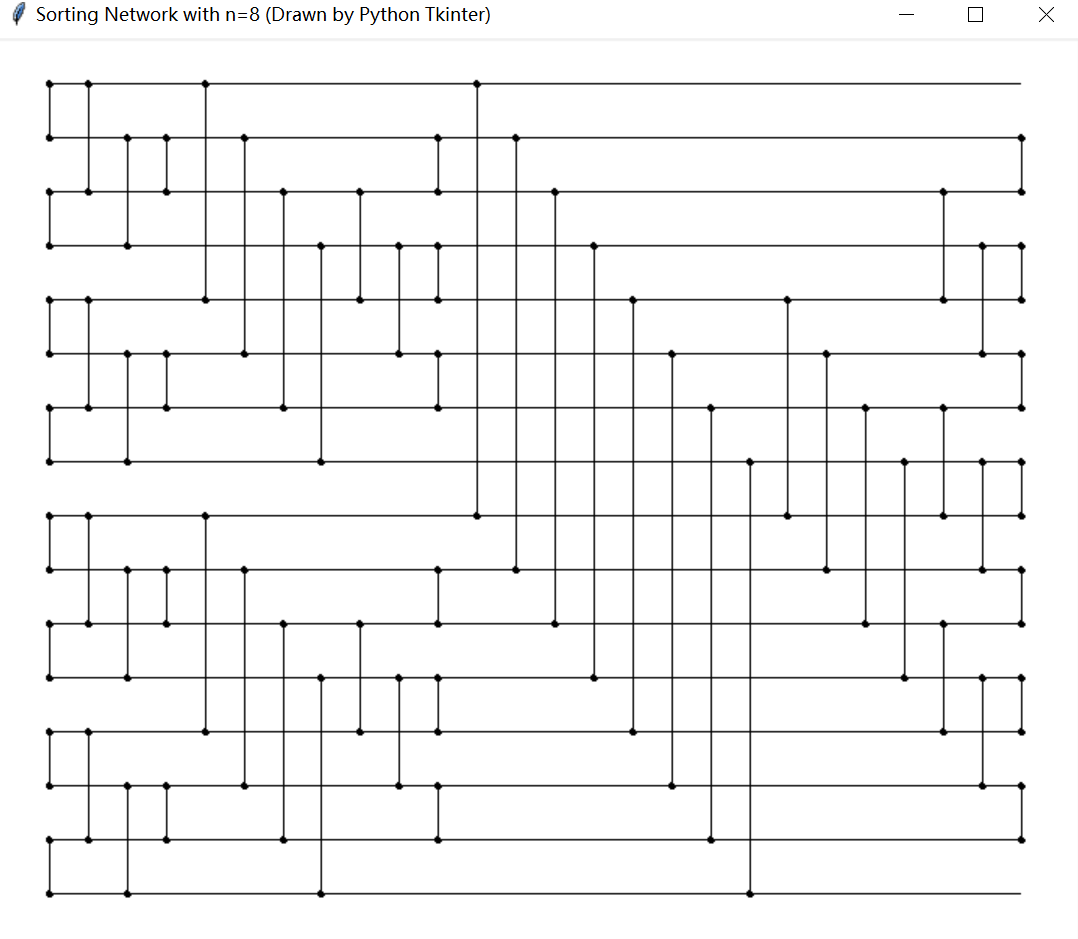
\includegraphics[width=12cm]{8.PNG}
			\caption{Picture for n=8 }
			\label{fig1}
		\end{figure} 
	 \begin{figure}[htbp]
		\centering
		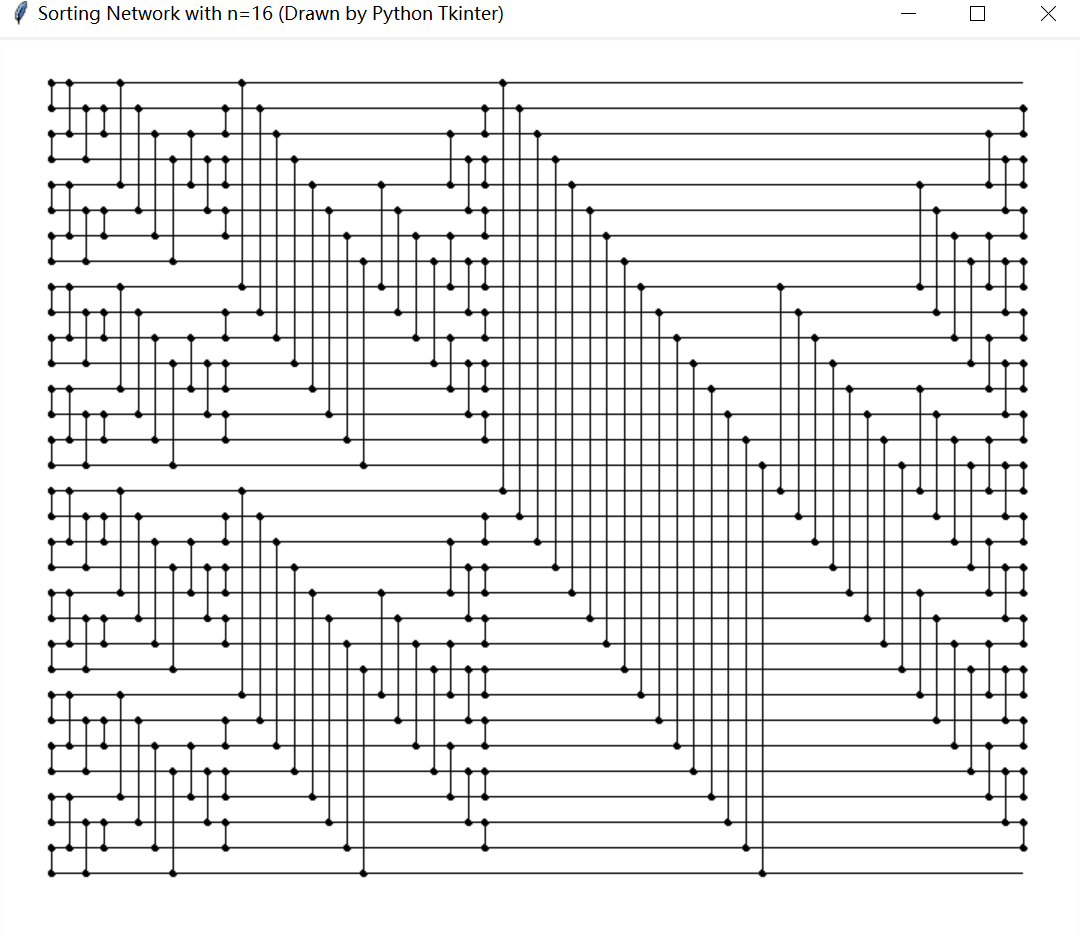
\includegraphics[width=12cm]{16.PNG}
		\caption{Picture for n=16 }
		\label{fig2}
			\end{figure} 
		
		\begin{figure}[htbp]
			\centering
			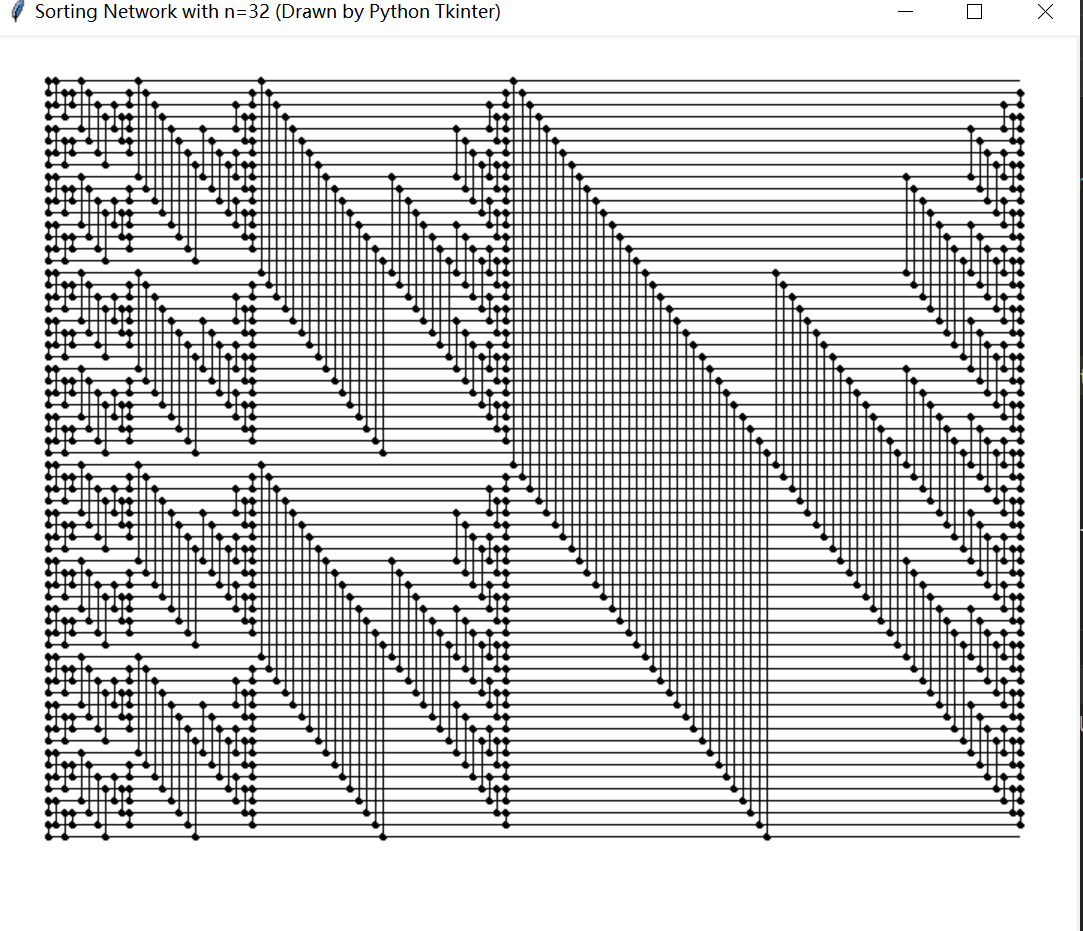
\includegraphics[width=12cm]{32.PNG}
			\caption{Picture for n=32 }
			\label{fig3}
		\end{figure} 
	
	\begin{figure}[htbp]
		\centering
		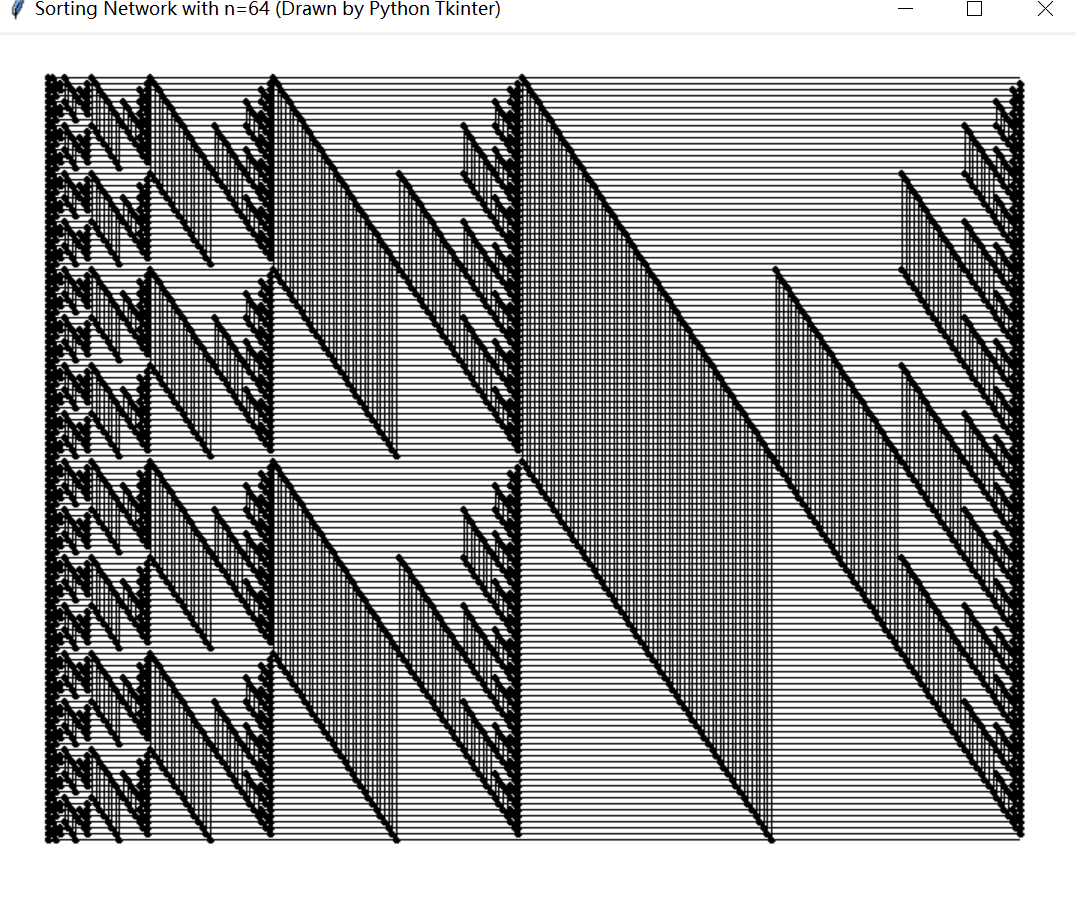
\includegraphics[width=12cm]{64.PNG}
		\caption{Picture for n=64}
		\label{fig4}
	\end{figure} 


	(b) When we deal with a sorting problem with 2n number, we should get two n-sorted array and then do the 2n-array merge.
	So we can just work on the depth of the 2n-merging, and then do recursive calculation to get the total depth.
	
	When merging 2n elements, we should merge two n-array and then combine them. Keep doing this until there are 1-arrays which don't need division.Considering that the combinations can be parallel, we can get the depth of n-merging: $\log 2n $.
	
	Then, about the total depth:
	$$depth=\log 2n + \log n+\log {\frac{n}{2}}+\log {\frac{n}{4}+\cdots+\log 2+\log 1}  $$
	$$depth=\frac{(1+\log{2n})*\log{2n}}{2}$$
	So, the depth of a 2n-input odd-even sorting network is $O(\log^2 n)$.
	
	(c) First we need to introduce the domain conversion lemma, which says if a merging net work transform the input $\textbf{a}=<a_1,a_2,\cdots,a_n>$ and $\textbf{b}=<b_1,b_2,\cdots,b_n>$into the output sequence $\textbf{c}=<c_1,c_2,\cdots,c_n>$,then for any monotonically increasing function $f$, the network transforms the input sequence $f(\textbf{a}),f(\textbf{b})$ to $f(\textbf{c})$.
	
	Now, prove the introduced lemma by induction:
	
	\textbf{Basis.} When there is only one element in both input sequences, it is obvious that the lemma is correct.
	
	\textbf{Assumption} If a wire assumes the value $i$ (from \textbf{a} or \textbf{b}), then it assumnes the value $f(i)$ (from f(\textbf{a}) or f(\textbf{b})).
	
	\textbf{Inducion} A comparator at depth $d\geq$1 disposes the input from the depth $d_i<d$. By assumtion the output at depth $d_i$ should be transformed from $i,j$ to $f(i)$ and $f(j)$, then the comparator at depth $d$ will dispose the $f(i)$ and $f(j)$. If $i$ is smaller, then the $f(i)$ will be smaller and take the place of $i$. Then, the lemma is proved.
	
	Then we can see that the zero-one principle applies to this case.(The continuing proof is similar to that in class).
	
	Then, we will use the zero-one principle and  prove the correctness for zero-one sequences.
	
	Conclude the operations for a 2n-input ($<a_1,a_2,a_3,\cdots,a_n>$and $<a_{n+1},\cdots,a_{2n}>$) as 4 steps :
	
	(1) Divide the 2n-inputs into two $\frac{n}{2}$-odd groups and two $\frac{n}{2}$-even groups.
	
	(2) Merge the two $\frac{n}{2}$-odd groups($<a_1,a_3,\cdots>$and$<a_{n+1},a_{n+3},\cdots>$) into a n-odd group 
	
	(3) Parallelly merge the two $\frac{n}{2}$-even groups($<a_2,a_4,\cdots>$and$<a_{n+2},a_{n+4},\cdots>$) into a n-even group
	
	(4) Combine the n-odd group and the n-even group by comparing and adjusting between the $a_{2i}$ and $a_{2i+1}$.
	
	Then we will prove the correctness of the network by induction.	

	
   \textbf{Basis.} It is easy to see, when k=1, the input is 2, the network for 2-input is correct.
   
	\textbf{Assumption} For any k=n/2, the input is k, the network is correct.
	
	\textbf{Inducion} When k=n, we need to prove the correctness:
	  
	  Because of the assumption, the step(2)(3) can be finished correctly, then we just need to prove the step(4):
	  
		We can see that the first element in n-odd (n-even) group must be the $a_1$ or $a_{n+1}$ ($a_2$ or $a_{n+2}$). Then because $a_1\leq a_2$ and $a_{n+1}\leq a_{n+2}$, the first element in final 2n-output (called \textbf{c}) must be from the n-odd group. So, to get the final sequence, there is no need to compare the $c_1$ and $c_2$. With the same reason, there is no need to compare the $c_3$ and $c_4$, $c_5$ and $c_6$ and so on.
	
	Therefore, we just need to compare and adjust the $c_2$ and $c_3$, $c_4$ and $c_5$ and so on, which is exactly what the step (4) does. So, we can see the correctness of step(4). 
	 
	
	Then the correctness is finally proved. 
	
	PS: The last proof needn't use 0-1 sequence, but because the process is kind of abstract, 0-1 sequence can be used to help simplify the question, which will not affect the result because of the 0-1 principle.
	
	\end{solution}
   


\end{enumerate}

\vspace{30pt}


\textbf{Remark:} You need to include your .pdf, .tex and .py files (or other possible sources) in your uploaded .rar or .zip file.

%========================================================================
\end{document}
